\documentclass{beamer}

\mode<presentation>{
\usetheme{Madrid}
%\usecolortheme{beaver}
}
\usepackage[utf8]{inputenc}
%\usepackage{default}
%\usepackage[portuguese]{babel}
%\usepackage{pgfplots}
%\pgfplotsset{/pgf/number format/use comma,compat=newest}
%\usepackage{color}
\usepackage{amsfonts}
\usepackage{mathrsfs}  

%\usepackage{hyperref}


%MEUS COMANDOs

\usepackage{tikz}
\usetikzlibrary{quotes, angles, intersections}
\newcommand{\R}{\mathbb{R}}
\newcommand{\D}{\mathscr{D}}
\newcommand{\Pp}{\mathscr{P}}
\newcommand{\Cc}{\mathscr{C}}
\newcommand{\E}{\mathscr{E}}

\newcommand{\bigO}{\mathscr{O}}

\usepackage{pgfplots}
\pgfplotsset{compat=1.4}
%\usepgfplotslibrary{external}
%\tikzexternalize



%FIM MEUS COMANDOS

\title[Qualificação de Mestrado]{Planar Maximal Covering with Ellipses}
\author[Tedeschi, D. F.]{Danilo F. Tedeschi}
\institute[ICMC]{Instituto de Ciências Matemáticas e Computação}
\date{\today}

\begin{document}

\begin{frame}
 \maketitle
\end{frame}

\begin{frame}
\frametitle{Contents}
 \tableofcontents
\end{frame}

\section{Introduction}
\begin{frame}
\frametitle{Introduction}
\begin{itemize}
	\item Covering problems
	\begin{itemize}
		\item Set Cover Problem
		\item Maximal Covering Problem
	\end{itemize}
	\item Maximal Covering Location Problem (MCLP)
	\item Planar Maximal Covering Location Problem (PMCLP)
	\begin{itemize}
	\item One disk: $\bigO(n^2)$ and $\bigO(n^2\log{n})$ algorithms
	\item $m$ disks: $\bigO(n^{2m-1}\log{n})$ algorithm
	\end{itemize}
	\item Goals
	\begin{itemize}
		\item Develop a $\bigO(n^2\log{n})$ algorithm for the one disk case
		\item Adapt it for the $m$ ellipses case
	\end{itemize}
\end{itemize}

\end{frame} 


\section{Preliminaries}

\begin{frame}{Preliminaries}
	
	\begin{block}{Norms}
		Let $u \in \R^2$ and $Q$ a $2x2$ positive definite matrix
		\begin{itemize}
			\item Euclidean
			\begin{equation*}
			||u||_2 = \sqrt{u^Tu}
			\end{equation*}
			
			\item Elliptical
			\begin{equation*}
			||u||_{Q} = \sqrt{u^TQu}
			\end{equation*}
		\end{itemize}
	\end{block}

\end{frame}

\begin{frame}{Preliminaries}
	\begin{figure}[H]
		\centering
		
		\caption{The elliptical and euclidean norms.}
		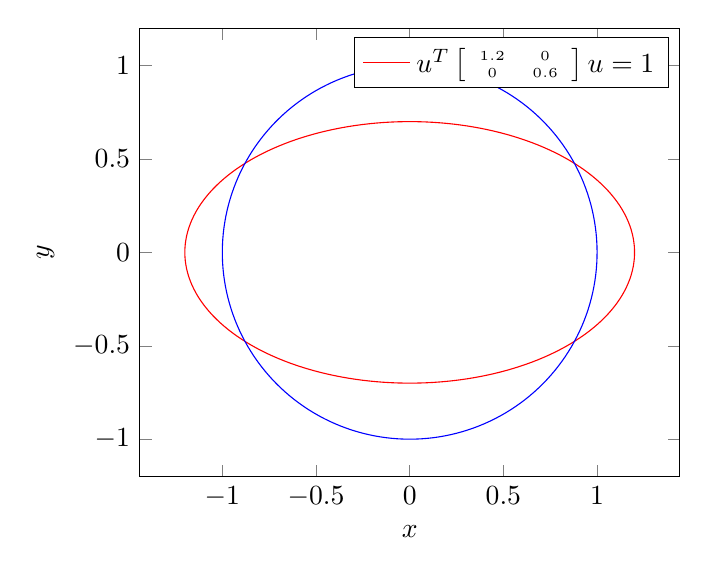
\begin{tikzpicture}
\begin{axis}[
    %axis lines = left,
    xlabel = $x$,
    ylabel = {$y$},
]
%Below the red parabola is defined
\addplot [domain=-pi:pi,samples=200,red]({1.2*cos(deg(x))}, {0.7*sin(deg(x))});

\addlegendentry{$\tiny u^T\left[\begin{array}{cc}
		1.2 & 0\\
		0 & 0.6
	\end{array}\right]u = 1$}
\addplot [domain=-pi:pi,samples=200,blue]({sin(deg(x))}, {cos(deg(x))});
\end{axis}
\end{tikzpicture}
		%\fautor
		\label{fig:3ellipses_intersect}
	\end{figure}
\end{frame}

\begin{frame}{Preliminaries}
	
	\begin{block}{Ellipse}
		Given a center $c \in \R^2$ and a $2x2$ p.d. matrix $Q$, an ellipse is the set of points that satisfy
		
		\begin{equation*}
		||u-c||_Q = 1,
		\end{equation*}
		
		with $\le$ representing the set of covered points
	\end{block}

	\begin{block}{Axis-parallel ellipse}
		Any $2$ by $2$ diagonal d.p. matrix determines an axis-parallel ellipse, which can also be described by
		
		\begin{equation*}
		\frac{(x-c_x)^2}{a^2} + \frac{(y-c_y)^2}{b^2} = 1,
		\end{equation*}
		
		where $(a,b)$ are the shape parameters and $c=(c_x,c_y)$ is the center.
	\end{block}

\end{frame}



\section{Maximal Covering by Disks}
\begin{frame}{Maximal Covering by Disks}{One disk}
	
	$MCD(\Pp, 1)$ is the problem of placing one disk on the plane to cover a subset of a demand set $\Pp$ maximizing the weights of the covered points.
	
	\begin{equation*}\label{eq:max_one_disk}
		\max_q w(\Pp \cap D(q)),
	\end{equation*}
	
	\begin{itemize}
		\item $\Pp=\{p_1,\dots,p_n\}$ is the demand set with weights $w(p_i)>0$
		\item $w(A)$, $A\subset \Pp$, is the sum of weights of the points in $A$
		\item $D(q)$ is a unit disk with center at point $q$
		\item We will introduce an equivalent problem...
	\end{itemize}
\end{frame}

\subsection{Maximum Weight Clique Problem}
\begin{frame}{Maximum Weight Clique Problem}
	Let $\D=\{D_1,\dots,D_n\}$ be a set of $n$ unit disks with weights $w_i>0$. The maximum weight clique is defined as
	
	\begin{equation*}
	\max_q \sum_{D_k \cap q \neq \emptyset} w_k,
	\end{equation*}
	
	\begin{itemize}
		\item The disks are fixed with centers at $\Pp =\{p_1,\dots,p_n\}$ with $w_k=w(p_k)$
		\item A clique is a non-empty intersection area of a subset of disks. We search for only a point in an optimal clique.
		\item An optimal solution for the maximum weight clique is an optimal solution for $MCD(\Pp,1)$.
	\end{itemize}
\end{frame}

\begin{frame}{Maximum Weight Clique Problem}{Equivalence}
		\begin{figure}[H]
		\centering
		
		\caption{An instance of $MCD(\Pp,1)$.}
		%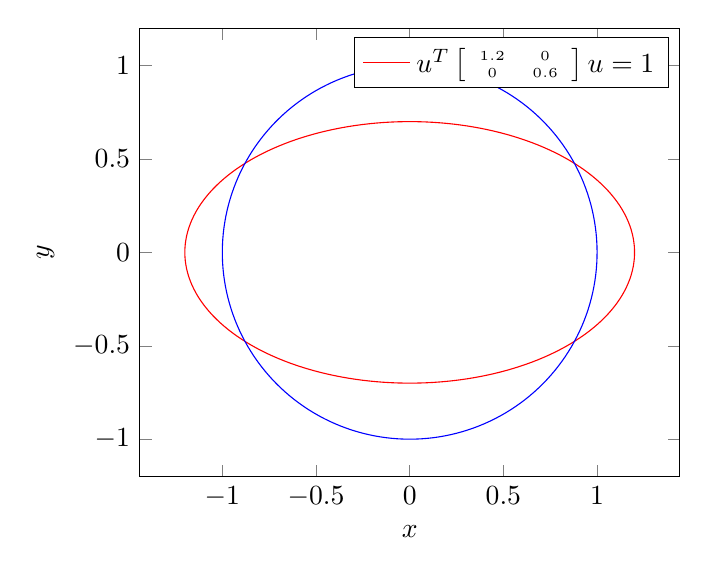
\begin{tikzpicture}
\begin{axis}[
    %axis lines = left,
    xlabel = $x$,
    ylabel = {$y$},
]
%Below the red parabola is defined
\addplot [domain=-pi:pi,samples=200,red]({1.2*cos(deg(x))}, {0.7*sin(deg(x))});

\addlegendentry{$\tiny u^T\left[\begin{array}{cc}
		1.2 & 0\\
		0 & 0.6
	\end{array}\right]u = 1$}
\addplot [domain=-pi:pi,samples=200,blue]({sin(deg(x))}, {cos(deg(x))});
\end{axis}
\end{tikzpicture}
      \center{\includegraphics[width=.7\textwidth]{figures/mcd_instance.png}}
		%\fautor
		\label{fig:mcd_instance}
	\end{figure}
\end{frame}

\begin{frame}{Maximum Weight Clique Problem}{Equivalence}
	\begin{figure}[H]
		\centering
		
		\caption{An instance of $MCD(\Pp,1)$.}
		%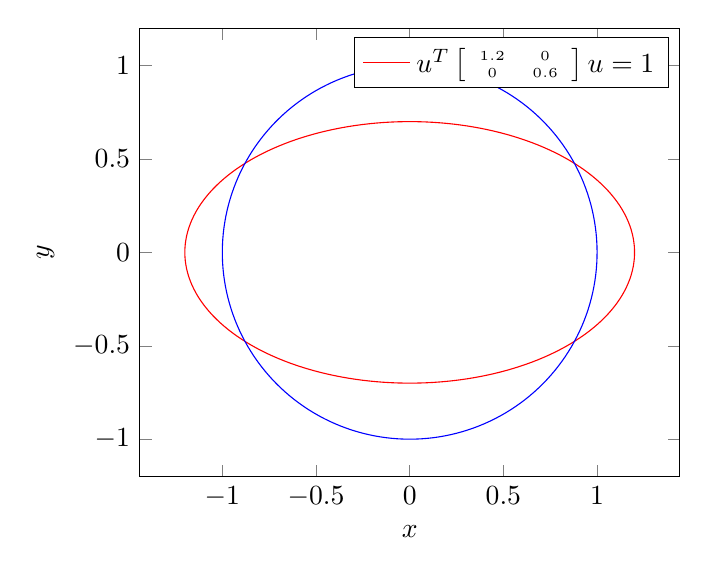
\begin{tikzpicture}
\begin{axis}[
    %axis lines = left,
    xlabel = $x$,
    ylabel = {$y$},
]
%Below the red parabola is defined
\addplot [domain=-pi:pi,samples=200,red]({1.2*cos(deg(x))}, {0.7*sin(deg(x))});

\addlegendentry{$\tiny u^T\left[\begin{array}{cc}
		1.2 & 0\\
		0 & 0.6
	\end{array}\right]u = 1$}
\addplot [domain=-pi:pi,samples=200,blue]({sin(deg(x))}, {cos(deg(x))});
\end{axis}
\end{tikzpicture}
		\center{\includegraphics[width=.7\textwidth]{figures/mwc_instance.png}}
		%\fautor
		\label{fig:max_wieght_clique}
	\end{figure}
\end{frame}

\begin{frame}{Maximum Weight Clique Problem}{Algorithm}
	Let $\Gamma_+(i,j)$ and $\Gamma_-(i,j)$ be the opening and closing angles of intersections of disks $i$ and $j$. Also, $\Gamma_+(i,j), \Gamma_-(i,j) \in [0,2\pi]$.
	\begin{figure}[H]
		\centering
		
		\caption{Three disks and their intersection points.}
		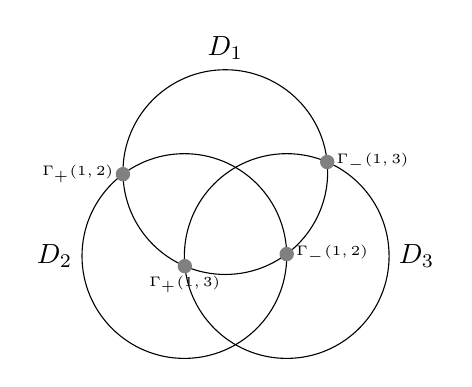
\begin{tikzpicture}[scale=1.3]
%\draw [help lines] (-5,-3) grid (5,3);

\draw[name path = c1] (0,0) circle (1cm);
\draw[name path = c3] (0.6,-0.82) circle (1cm);
\draw[name path = c2] (-0.4,-0.82) circle (1cm);

\node[above] at (0, 1) {$D_1$};
\node[left] at (-1.4, -0.82) {$D_2$};
\node[right] at (1.6, -0.82) {$D_3$};

\path [name intersections={of=c1 and c3}] ;
\foreach \i in {1,...,2}
\fill [color=gray] (intersection-\i) circle (2pt) ;

\node[right] at (intersection-1) {\tiny $\Gamma_-(1,3)$};
\node[left, below] at (intersection-2) {\tiny $\Gamma_+(1,3)$};

\path [name intersections={of=c1 and c2}] ;
\foreach \i in {1,...,2}
\fill [color=gray] (intersection-\i) circle (2pt) ;

\node[left] at (intersection-1) {\tiny $\Gamma_+(1,2)$};
\node[below,right] at (intersection-2) {\tiny $\Gamma_-(1,2)$};

%\draw [-] (-5,0) -- (5,0);
%\draw [-] (0,-3) -- (0,3);
%\draw [|-|] (0.001,-0.1) -- (4.999,-0.1);
\end{tikzpicture}
		%\fautor
		\label{fig:3disks_intersect}
	\end{figure}
\end{frame}

\begin{frame}{Maximum Weight Clique Problem}{Algorithm}
	For a disk $D_i$, a counter-clockwise traversal visits every $\Gamma_+(i,j)$ and $\Gamma_-(i,j)$ in counter-clockwise order.
	
	\begin{itemize}
		\item An intersection region of disks is bounded by arcs.
		
		\item The arc $\Gamma_+(i,j),\Gamma_-(i,j)$ (counter-clockwise) determines a region where $i$ and $j$ intersect.
		
		\item In a counter-clockwise traversal, the arcs where $\Gamma_+(i,j) > \Gamma_-(i,j)$ can be a problem for the implementation. Work-around: repeat it.
	\end{itemize}
\end{frame}

\begin{frame}{Maximum Weight Clique Problem}{Algorithm}
	
	The algorithm is described simply as:
	
	For every disk, traverse the sorted list of intersection angles twice, keeping a set of active disks, and the current best solution.
	
\begin{figure}[H]
	\centering
	
	\caption{The intersections list of a disk with three other disks.}
	\input{figures/fig:array_disks.tex}
%	\fautor
	\label{fig:array_disks}
\end{figure}
\end{frame}


\begin{frame}{Maximum Weight Clique Problem}{Algorithm}
	
	The run-time complexity of the algorithm is $\bigO(n^2\log{n})$.
	
	\begin{itemize}
		\item There are $\bigO(n^2)$ intersections among $n$ disks
		
		\item Sorting takes $\bigO(n^2\log{n})$
		
		\item The traversal takes $\bigO(n)$ for every disk.
		
		\item Can be implemented in $K\log{n}$ where $K$ is the number of intersections. 
	\end{itemize}

\begin{block}{Multiple disks}
	For every disk, try every possible assignment that the traversal goes through.
\end{block}
	

	
	
\end{frame}

\section{Maximal Covering by Ellipses}

\begin{frame}{Maximal Covering by Ellipses}
	content... trabalhos passados
\end{frame}

\begin{frame}{Cobertura Maximal por Ellipses}{$m$ elipses}
	content... algoritmo
\end{frame}

\section{Trabalhos Futuros}

\begin{frame}{Trabalhos Futuros}

\end{frame}
\end{document}